\subsection{Knochenschallaktor} \label{sec:knochenschallaktor}

Nachdem das vom Mikrocontroller ausgegebene Audio-File über die Verstärkerstufe entsprechend aufbereitet wurde, kann nun die Audiodatei über einen sogenannten Knochenschallaktor ausgegeben werden.
Der Aktor arbeitet nach dem Prinzip der Weiterleitung von Schall-Schwingungen oder auch Vibrationen. Dadurch lässt sich der ursprüngliche Gehörgang umgehen und die Schwingungen werden über den Schädelknochen an das Innenohr übertragen. Dies verbessert auch die Hygiene der Anwendung, da kein direkter Kontakt mit dem Gehörgang stattfindet.\cite{Knochenschall}
Für die Anwendung im Dōjō wird ein Knochenschallaktor des Herstellers Adafruit verwendet, welcher in der Abbildung \ref{fig:knochenschallAda} ersichtlich ist.

\begin{figure}[htbp]
	\centering
	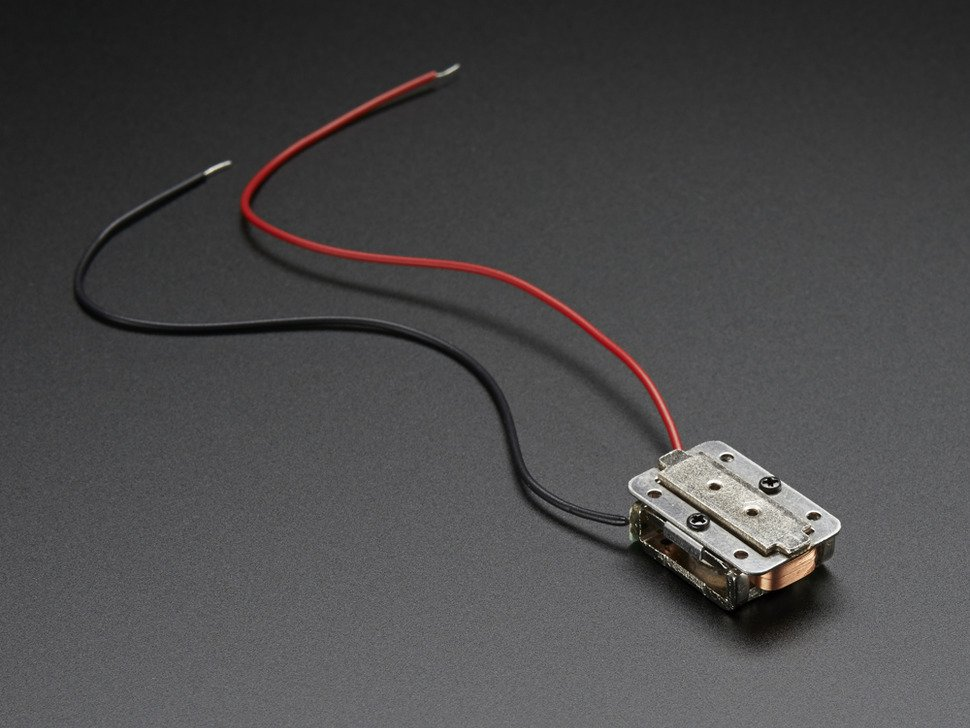
\includegraphics[width=0.5\textwidth]{Data/KnochenschallaktorAdafruit1}
	\caption[Knochenschallaktor \cite{BoneConductorAdafruit}]{Knochenschallaktor von Adafruit}
	\label{fig:knochenschallAda}
\end{figure} 

Das ausgewählte Bauteil eignet sich bestens für die Verwendung im Dōjō. Mit einem Gewicht von 9.6 g und den Dimensionen 14x21,5x7,9 lässt sich der Aktor gut in das bestehende Gehäuse implementieren \cite{BoneConductorAdafruit}. Weiter ist das Bauteil relativ kostengünstig im Handel erhältlich und kann $1W_{RMS}$ Leistung liefern, was sich dann in der Lautstärke bemerkbar macht. Nach ausführlichen Recherchearbeiten konnten keine wirklichen Alternativen ausgemacht werden. Meist befindet sich die Technologie noch in der Entwicklungsphase oder fällt aufgrund des Preises aus der Auswahlmöglichkeit.